\chapter{System overview}
\label{chap:systoverview}
%Short introduction to system context and design. Background of the project
A description of the \applicationname{} can be found in the URD \cite{urd}. Furthermore, the SRD \cite{srd} includes descriptions of the background of \projectname{} and the environment it operates in.
\projectname{} is a web-based information system. It does not interact with any other information systems in its environment. Figure \ref{fig:environment} shows the environment of \projectname{}.

\begin{figure}[h!]
\begin{center}
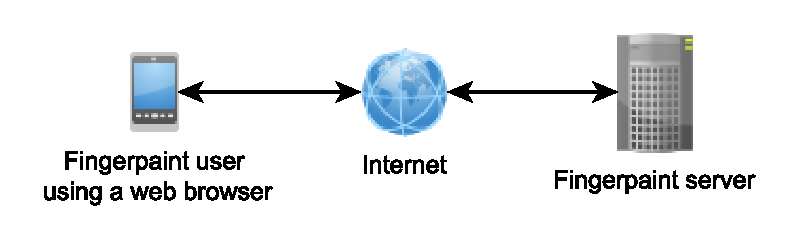
\includegraphics[keepaspectratio=true,width=0.8\textwidth]{Environment.pdf}\captionof{figure}{The environment of \projectname \label{fig:environment}}
\end{center}
\end{figure}

\section{Design decisions}
\label{sec:designdecisions}
The architecture of the \applicationname{} has mostly been determined by the customer. The goal of this project is to build a cross platform application, that also runs on touch devices. Furthermore, the code to run a simulation is quite heavy and therefore the client has asked us to let the simulation run on the server-side. These two design decisions are very important for how the application behaves, but they are not made by us, they are made by the client.

On the server-side, the simulation code which is implemented in Fortran communicates with our server-side code which is implemented in Java through JNI (via a small C wrapper program). It would have been possible to use sockets for this, but we chose for JNI because it was more straightforward to implement.

The client has requested to support saving and loading of distributions, protocols and results on the client-side. For this, we use \emph{local storage}, which is a HTML5 feature. Note that there are currently no real alternatives for this.